Ring signatures, introduced by Rivest, Shamir and Tauman, \cite{AC:RivShaTau01}, allow to anonymously sign a message on behalf of a ring of users $P_1,\ldots,P_n$, only if the signer belongs to that ring. Although there are other cryptographic schemes that provide similar guarantees (e.g.~group signatures \cite{EC:ChaVan91}), ring signatures are not coordinated: each user generates secret/public keys on his own -- i.e.~no central authorities -- and might sign on behalf of a ring without the approval or assistance of the other members.

While the more efficient constructions have signature size logarithmic in the size of the ring \cite{EC:GroKoh15,EC:LLNW16}, all of them rely on the {random oracle model}.
Without random oracles all constructions have signatures of size linear in the size of the ring, being the sole exception the $\Theta(\sqrt{n})$ ring signature of Chandran et al.~\cite{ICALP:ChaGroSah07}. 
We remark that no asymptotic improvements to Chandran et al.'s construction have been made since their introduction (only improvements in the constants by R\`afols \cite{TCC:Rafols15} and by Gonz\'alez et al.~\cite{AC:GonHevRaf15}). Although some previous works claim to construct signatures of constant \cite{ACISP:BosDasRan15} or logarithmic \cite{IET:GriSusPla16} size, they are either in a weaker security model or we can identify a flaw in the construction (see Section \ref{sec:rs-flawed}). 

In this work we present the first ring signature (without random oracles) whose signature size is asymptotically smaller than Chandran et al.'s. Our ring signature consists of $\Theta(\sqrt[3]{n})$ group elements, computing a signature requires $\Theta(\sqrt[3]{n})$ exponentiations, and verifying a signature requires $\Theta(n^{2/3})$ pairings.

The security of our construction relies on a security assumption -- the {permutation pairing assumption} -- introduced by Groth and Lu \cite{AC:GroLu07} in an unrelated setting: proofs of correctness of a shuffle. While the assumption is ``non-standard'', in the sense that is not a ``DDH like'' assumption, it is a falsifiable assumption and it was proven hard in generic symmetric groups by Groth and Lu. For simplicity, we work on symmetric groups ($\GG_1=\GG_2$) but our techniques can be easily extended to asymmetric groups as we show in Appendix \ref{sec:aPPA}.

Our ring signature outperforms Chandran et al.'s in terms signature size for any $n > 246$, in terms of signature generation time for any $n>205$, and in terms of verifier efficiency for any $n>170$. However, this analysis should be taken with care, since Chandran et al.'s signature is proven secure under the decisional linear (DLin) assumption while ours is proven secure under the permutation pairing assumption. Therefore, it could be the case that our scheme would be as secure as Chandran et al.'s at higher values of the security parameter. In Table \ref{table:eff} we provide a comparison between our scheme and Chandran et al.'s.

\begin{table}[h]
\begin{center}
\begin{minipage}{\textwidth}
\begin{center}
%\begin{scriptsize}
\begin{tabular}{|l|l|l|}
\hline
                                           & Chandran et al.~\cite{ICALP:ChaGroSah07} & This work \\
\hline\hline
\rule{0pt}{2.5ex}CRS size                  & $9$                                       & $9$       \\ 
\rule{0pt}{2.5ex}Verification key size     & $1$                                       & $5$       \\
\rule{0pt}{2.5ex}Signature size            & $24 \sqrt{n} + 24$                        & $39 \sqrt[3]{n} + 30 \sqrt[6]{n} + 81$\\    
\rule{0pt}{2.5ex}Signature generation time & $42 \sqrt{n} + 49$                        & $69 \sqrt[3]{n} + 42 \sqrt[6]{n} + 142$\\
\rule{0pt}{2.5ex}Verification time         & $3 n + 120 \sqrt{n} + 121$                & $6 n^{2/3} + 210 \sqrt[3]{n} + 186 \sqrt[6]{n} + 411$\\
\hline 
\end{tabular}
%\end{scriptsize}
\end{center}
\caption{Comparison of Chandran et al.'s ring signature and ours for a ring of size $n$. 'Signature generation time' is measured in number of exponentiations, 'Verification time' is measured in number of pairings, and all other rows are measured in number of group elements.\label{table:eff}}
\end{minipage}
\end{center}
\end{table}

%
%\begin{figure}[!t]
%	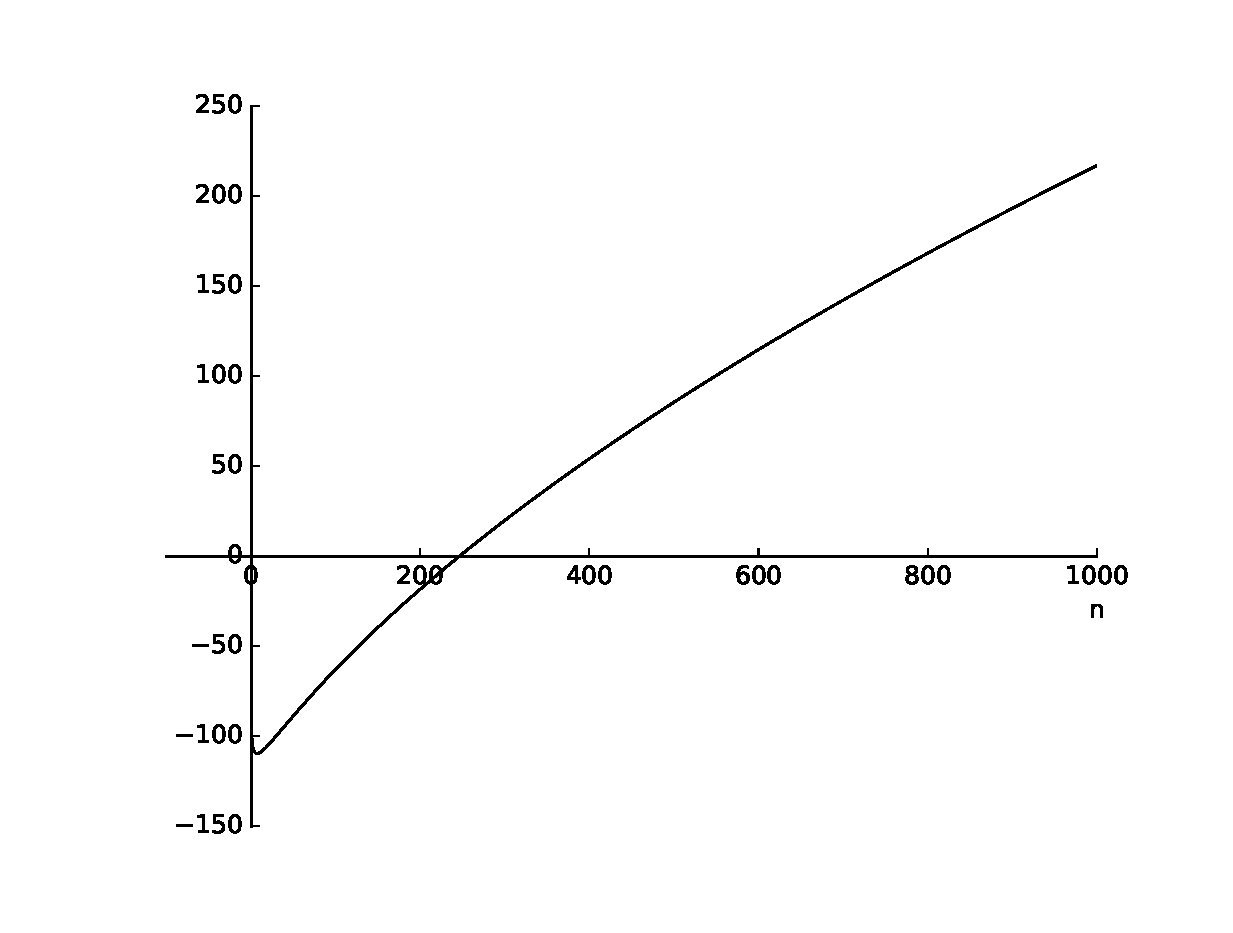
\includegraphics[scale=.25]{intro/sign_size}
%	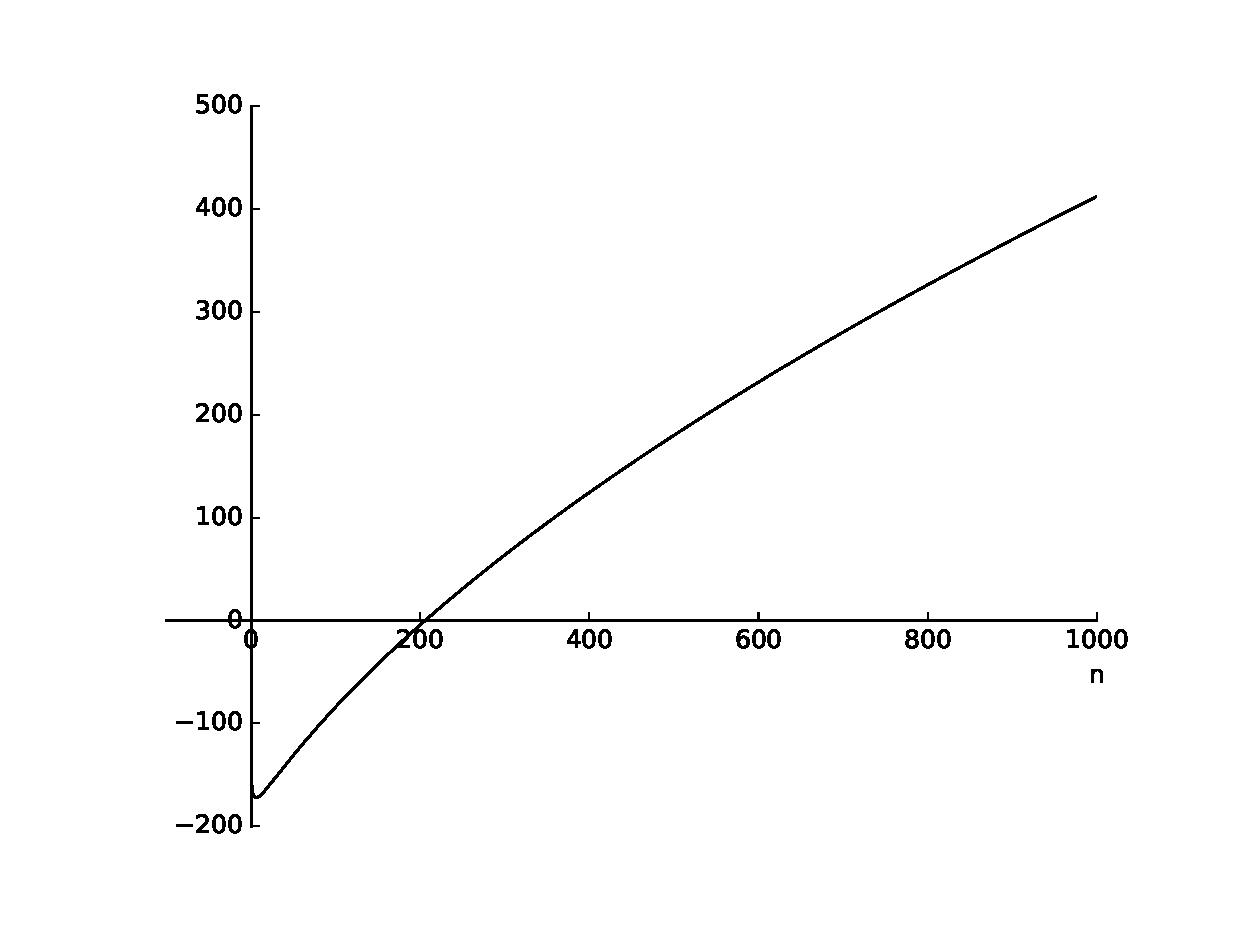
\includegraphics[scale=.25]{intro/sign_time}
%	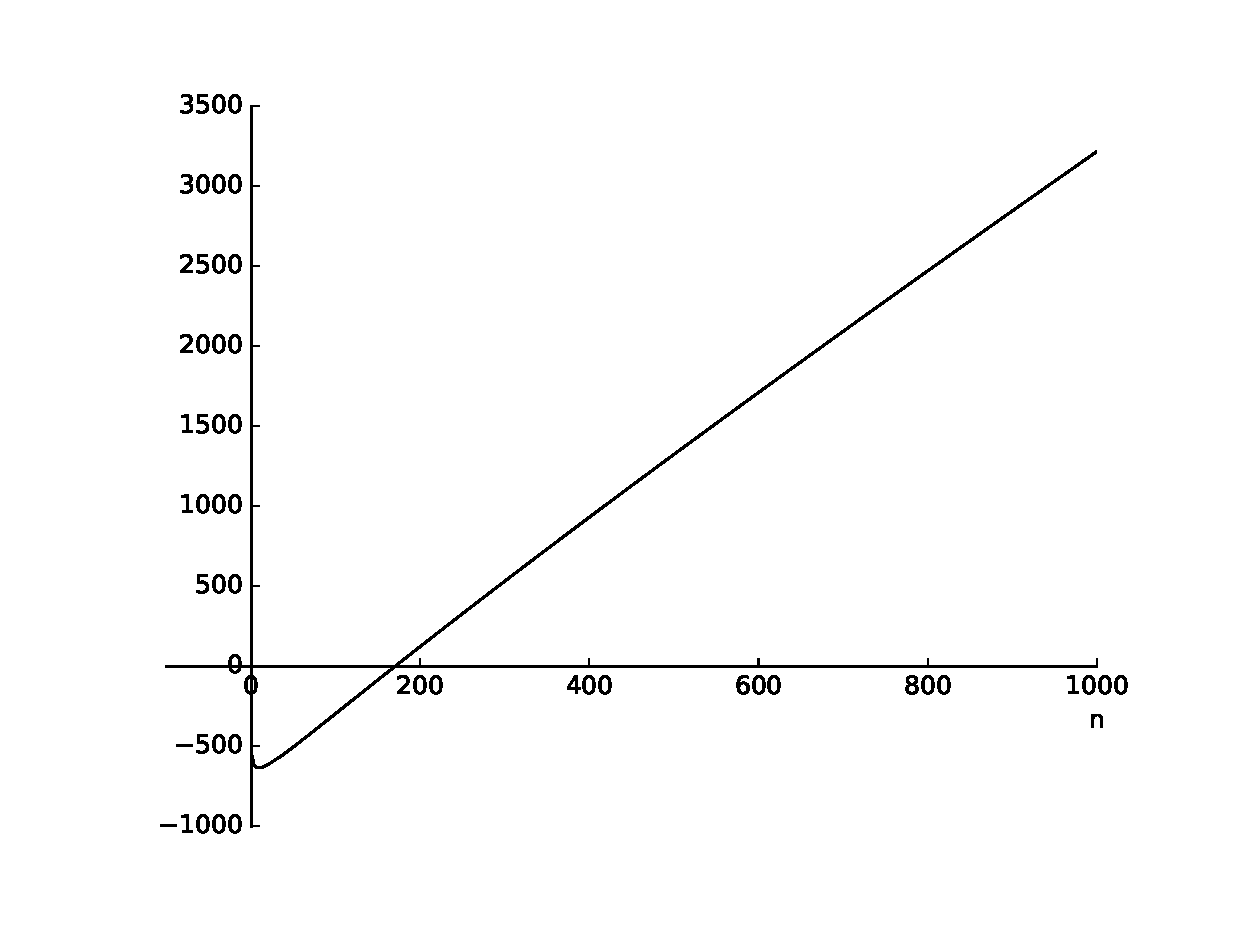
\includegraphics[scale=.25]{intro/ver_time}
%\end{figure}

\subsection{Technical Overview}
Consider a symmetric bilinear group $gk:=(\GG,\GG_T,e,\mathcal{P},q)$ of prime order $q$, where $\mathcal{P}$ is a generator of $\GG$. Define $[x]=x\mathcal{P}$ for any $x\in\mathbb{Z}_q$.  We will write all group operations using additive notation.

Our main technical tool is a structure preserving -- i.e.~compatible with Groth-Sahai proofs -- hash function with \emph{always second-preimage resistance} (aSec in the terminology of Rogaway and Shrimpton \cite{FSE:RogShr04})
\begin{align*}
h : Q_m &\to \GG^2\\
      A &\mapsto h(A) := \sum_{[\vecb{a}]\in A} [\vecb{a}],
\end{align*}
 where
$$
Q_m:= \{A\subset\GG^2: |A|=m \text{ and }\forall [\vecb{a}]\in A, e([a_2],[1])=e([a_1],[a_1])\}.
$$
That is, for a randomly chosen $A\in Q_m$, it is computationally infeasible to find a different $A'\in Q_m$ such that and $h(A)=h(A')$. The hardness of finding second preimages for $h$ is a direct consequence of the permutation pairing assumption introduced by Groth and Lu \cite{AC:GroLu07}.

We consider also the family of collision resistant hash functions parametrized by $[\matr{A}]\in\GG^{2\times m}$
\begin{align*}
g_{[\matr{A}]} : \GG^m &\to \GG^2\\
           [\vecb{x}] &\mapsto g_{[\matr{A}]}([\vecb{x}]) = [\matr{A}\vecb{x}]
\end{align*}
Given $[\matr{A}],[\matr{A}']\in\GG^{2\times m}$ define $A,A'$ as the sets whose elements are the columns of, respectively, $[\matr{A}]$ and $[\matr{A}']$. Then $g_{[\matr{A}]}([\vecb{x}]) = g_{[\matr{A}']}([\vecb{x}'])$ and $A=A'$ implies that there is a permutation $\pi$ such that $[\vecb{x}]=\pi([\vecb{x}'])$ unless $[\vecb{x}],\pi([\vecb{x}'])$ is a collision for $g_{[\matr{A}]}$.
 
 Finding collosions for $g_{[\matr{A}]}$ is as hard as finding a non-zero element in the kernel of $[\matr{A}]$, since
$$
g_{[\matr{A}]}([\vecb{x}]) = g_{[\matr{A}]}([\vecb{x}']) \Longleftrightarrow [\matr{A}(\vecb{x}-\vecb{x}')]=[0],
$$
which is in general a hard problem.
Morillo et al.~\cite{AC:MorRafVil16} formally defined this computational (or search) problem as the kernel matrix Diffie-Hellman assumption (KerMDH) and it has many applications such as constructing constant size QA-NIZK proofs of membership in the linear span of a matrix \cite{EC:LPJY14,EC:KilWee15}. Morillo et al. proved the hardness of the KerMDH assumption in generic bilinear groups for many distributions of $[\matr{A}]$, and for some specific distributions (e.g.~the uniform distribution) it can be proven harder than the decisional linear assumption. If $A$ is randomly chosen from $Q_m$, then finding an element on the kernel of $[\matr{A}]$ was proven hard in generic bilinear groups by Groth and Lu \cite{AC:GroLu07} (although using a different terminology).

\subsubsection{High level description.}
Our scheme follows the ring signature of Chandran et al.~and improves the underlying $\Theta(\sqrt{n})$ proof that the Groth-Sahai commitment of a Boneh-Boyen signature verification key $[vk]\in\GG$ belongs to the ring of verification keys $R=\{[vk_1],\ldots,[vk_n]\}$. In the rest of this section we simply refer to this proof as a ``set-membership proof'' and we remark that it might be applied to any set of group elements (not only of verification keys).

We enlarge the verification key by including $[\vecb{a}]\gets Q_1$ and $sk[\vecb{a}]=\vecb{a}[vk]$, where $[vk]$ is the verification key of Chandran et al.'s scheme and $sk=vk$ is the secret key (recall that $vk$ is the discrete logarithm of $[vk]$). In spite of this difference, our proof also show that a Boneh-Boyen verification key $[vk]$ is in the ring. 

Given the commitment of $[vk]=[vk_i]$, for some $1\leq i\leq n$, our proof consists of two set-mebership proofs in sets of size $\Theta(n^{2/3})$ (and thus each proof is of size $\Theta(\sqrt[3]{n})$) and $\Theta(\sqrt[3]{n})$ Groth-Sahai proofs and Groth-Sahai commitments. Let $1\leq \mu\leq m^2, 1\leq \nu \leq m$  such that $i=(\mu-1)m + \nu$, where $m:=\sqrt[3]{n}$. The prover and the verifier split the verification keys into $[\vecb{\kappa}_1],\ldots, [\vecb{\kappa}_{n^{2/3}}]$ such that $[\vecb{\kappa}_i] = ([vk_{(i-1)m+1}],\ldots,[vk_{im}])^\top\in\GG^m$ and also define $A_1,\ldots, A_{n^{2/3}}$, $[\matr{A}_1],\ldots, [\matr{A}_{n^{2/3}}]$ in a similar way.

The prover starts commiting to $h(A_\mu)$ and computes the first set-membership proof showing that $h(A_\mu)$ belongs the set $H:=\{h(A_1),\ldots,\allowbreak h(A_{n^{2/3}})\}$. Note that this set-membership proof requieres only $m$ group elements.
Let $[\matr{A}']$ the matrix whose first column is $[\vecb{a}_i]$ and the rest columns are the other columns of $[\matr{A}_\mu]$ (preserving the order). We indiviadually commit to each element of $A'=A_\mu$ and show using Groth-Sahai proofs that $A'\in Q_m$ and that $h(A')=h(A_\mu)$. From this part of the proof we get $m$ commitments to the elements of $A'$ and we know that, with all but negligible probability, $A'=A_\mu$.

Next, the prover computes Groth-Sahai commitments to each element of the vector $[\vecb{\kappa}']$, whose first element is $[vk_i]$ and the rest are the other verification keys in $[\vecb{\kappa}_\mu]$, and commits also to $g_{[\matr{A_{\mu'}}]}([\vecb{\kappa}_{\mu'}])$. The second set-membership proof shows that $g_{[\matr{A_{\mu'}}]}([\vecb{\kappa}_{\mu'}])$ belongs to the set $G:=\{g_{[\matr{A}_1]}([\vecb{\kappa}_1]),\allowbreak\ldots,g_{[\matr{A}_{n^{2/3}}]}([\vecb{\kappa}_{n^{2/3}}])\}$. (We also need to show that $\mu'=\mu$, which can be proven ``for free'' given the way Chandran et al.'s proof is constructed). Finally, the prover gives a Groth-Sahai proof that $g_{[\matr{A}']}([\vecb{\kappa}'])=g_{[\matr{A_{\mu'}}]}([\vecb{\kappa}_{\mu'}])$.

We conclude that $[\vecb{\kappa}']$ is a permutation of $[\vecb{\kappa}_\mu]$ and thus $[\kappa'_1]=[vk_i]$ is in the ring of verification keys.


